\chapter{Introduction}


The universe must be self-consistent. This is the basic premise physicists assume in the quest for the ultimate laws that govern our universe. Without it, a theory would be a mere description of a collection of observed facts. 

Despite highly precise experimental corroboration of the Standard Model of particle physics, which relies on Quantum Field Theory (QFT) with gauge symmetry, and Einstein's General Relativity (GR) that describes gravity, these two frameworks are mutually incompatible. That is without mentioning the foundational problems of QFT, that the Clay Mathematics Institute urges to solve with a million-dollar prize incentive\footnote{
See the link: \url{http://www.claymath.org/millennium-problems/yang\%E2\%80\%93mills-and-mass-gap} 
}.

Classical physics is elegantly formulated in terms of the least action principle. 
The standard procedure is to encode the dynamics in a quantity called action, 
minimize it with respect to the physical variables which gives a set of differential equations (of motion) to be solved. 
In quantum physics, we relax this principle. When quantizing a classical theory in Feynman path integral formulation, 
paths that do not minimize the action also contribute to the dynamics. In strong analogy with statistics, 
physical quantities are weighted observables $O$ by the exponential of the classical action\footnote{
The analogy is even closer when we analytically continue the time to pure imaginary time, i.e. Wick rotate $t \rightarrow -i t_{E}$, 
then the action becomes purely imaginary, and the exponential decays.}:
\[
 \braket{O} = \int D\phi \, O\, e^{-i S[\phi]/\hbar},
\]
where we used the shorthand notation $\phi$ for the collection of quantum fields\footnote{
Quantum mechanics can be formulated as a (0+1)-dimensional QFT.}. 
The problem is, however, the lack of a rigorous definition of the measure $D\phi$.
Very often, we only know how to compute quantum observables in certain limits, 
when we can rely on the saddle-point approximation to the integral. 
For example, in the classical limit (vanishing Plank constant $\hbar$), 
the saddle-point method for the partition function gives us the least action principle:
\[
 Z=\braket{1} \approx e^{-i S[\phi_c]/\hbar}; \quad  \delta S[\phi_c] = 0 .
\]
Other examples are the weak coupling limit, such as in Quantum Electrodynamics (QED), 
or the thermodynamic limit in quantum many-body systems. 
By contrast, we have no established analytical tool to handle strongly-coupled QFTs, 
which would explain quark confinement in Quantum Chromodynamics (QCD), and phases of high-Tc superconductors.

Only very few classes of path integrals are solvable. 
Besides free theories, path integrals of topological quantum field theories and some supersymmetric theories localize \emph{exactly} 
at their saddle-points. This highly non-trivial phenomenon is called the localization of path integrals, 
and it is one of the pillars our work is based on. 

Generalizing point-particles to strings, 
String Theory might be the best candidate for a consistent quantum gravity theory, 
which would be a unifying framework for QFT and GR. It is not free of mathematical problems though, 
for example the string action in a curved background is not fully known, 
and path integral measures are not rigorously defined either. Nevertheless, it is mathematically rich, 
with a web of dualities that connect different perturbative string theories (the underlying theory is known as the M-theory). 
It is offering us many insights otherwise unsuspected and a very important realization is the AdS/CFT correspondence. 
The most well-studied instance of the correspondence is the one between weakly-coupled superstring theory living on $AdS_5 \times S^5$ space, 
and a strongly-coupled supersymmetric conformal field theory (CFT) called $\mathcal{N}=4$  SYM. 
Despite much success (and still some issues concerning quantum stringy corrections), the correspondence remains an unproven conjecture.

An even more general correspondence is the gauge/string (or gauge/gravity) duality, 
also known as the holographic principle (so named because the gauge theory lives in a lower dimensional space than the string theory). 
If it were true, it would be revolutionary in many aspects. From a practical point of view,
on one hand we would have a toolbox to solve strongly-coupled gauge theories using essentially GR, 
and on the other hand, experiments on quantum gravity could be done in laboratories by handling systems like cold atoms. 
From a conceptual point of view, it could indicate that gravity, and hence spacetime, are emergent from lower dimensional quantum systems.

We lack the mathematical constructs to even formulate the conjecture in a precise manner. 
However, we can generalize what we learned from AdS/CFT to settings where we still hold some analytical control. 
A perfect toy model to investigate \emph{non-conformal} gauge/string duality is the unique massive deformation of $\mathcal{N}=4$ SYM, 
called $\mathcal{N}=2^*$ SYM.
On one hand, like $\mathcal{N}=4$ SYM, supersymmetric localization is applicable 
and reduces the complicated path integrals to a manageable matrix model,
allowing us to access its strongly-coupled regime (actually any finite coupling regime). 
On the other hand, $\mathcal{N}=2^*$ SYM 
is conjectured to be dual to a supergravity solution known as the Pilch-Warner background.
Figure \ref{fig:Overview} shows a graph on the relationship between different theories that we consider.
% Therefore, it is a golden opportunity to test the gauge/string duality beyond AdS/CFT, 
% and perhaps learn more about the string theory side through this duality. 


\begin{figure}[t]
\begin{center}
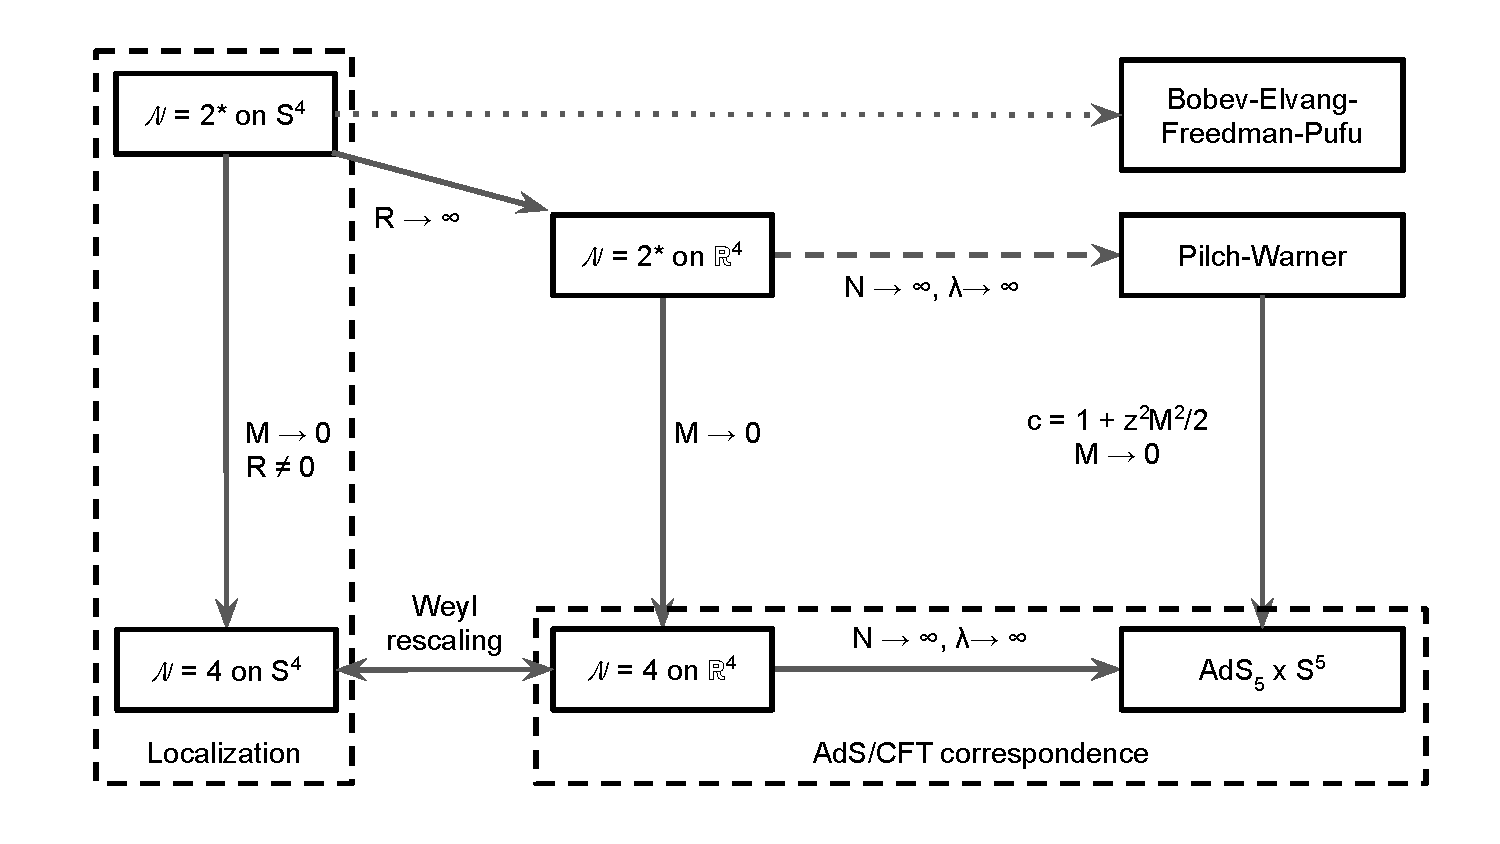
\includegraphics[width=\textwidth]{Images/Overview.pdf}
\end{center}
\caption{\label{fig:Overview} Localization applies to theories on the sphere, indicated by a dashed box. 
Since the gravity dual of $\mathcal{N}=2^*$ on $S^4$ is only partially known (indicated by the dotted line arrow), 
we take the decompactification limit ($R \rightarrow \infty$) to obtain $\mathcal{N}=2^*$ on $\mathbb{R}^4$.
Our research focuses on the dashed arrow,
which generalizes the well-established AdS/CFT correspondence shown in the dashed box below it. 
The limits will be explained through out the thesis.
%  in the 't Hooft limit ($N\rightarrow \infty$ and $\lambda \rightarrow \infty$), 
}
\end{figure}


\subsection*{Outline}
This thesis has two parts, both aimed at introducing and reviewing some background material in order to help the readers follow the appended papers.  
Part I focuses on the gauge theory side. We start off with the basics of the supersymmetric localization technique, 
then we go on to discuss the action of $\mathcal{N}=4$ SYM on $\mathbb{R}^4$ and on $S^4$. 
We then extend it to $\mathcal{N}=2^*$ SYM on $S^4$, and focus on the partition function after localization. 
We show the common technique to solve a matrix model, and conclude with the phase diagram of the theory. 
The last chapter of this part introduces the Wilson loop observables, and we review some known results in $\mathcal{N}=4$ case, 
and finally, write down the results we computed for $\mathcal{N}=2^*$ case. 
Part II starts with supergravity and some of its solutions, 
including $AdS_5\times S^5$ and Pilch-Warner. 
Then, we review the AdS/CFT correspondence and the logic behind its original derivation. In the end, we talk about holographic Wilson loops and connect our holographic solutions to the gauge theory results. 

\begin{quote}
 \emph{Physics is really nothing more than a search for ultimate simplicity, but so far all we have is a kind of elegant messiness.}
   ---  Bill Bryson
%  , \emph{A Short History of Nearly Everything}
\end{quote} 














